\chapter{Implementation}
\label{cha:implementation}

This section describes the actual implementation of the system, how it implements the different functionalities specified in previous sections and how these work together in order to realize the whole system. The different components of the system have been implemented independently with consultation and interface definitions during the development process, hence each component of the system is provided with its own dedicated section describing its implementation. Before the actual implementation is going to be put forward it is important to revisit the problem that the implementation shall cover and that is a "Maritime container IoT based monitoring system" capable of monitoring status and generating alarms for maritime containers while storing the alarms for historical purposes and also providing mobile interface to field technicians in order to monitor and resolve alarms. The complete system can be seen on the architectural diagram:

Whereas the previous chapter concerned itself with the overall plan in the abstract, this is where the actual experiment in the form of an implementation is taking form.  It is not the purpose of the implementation to fully realise the design described in the previous chapter. It is the exclusive purpose of the implementation (a subset of the design) to either validate or refute the hypotheses put forth
in the introduction. This, and nothing else. If it does less, you have posed questions you are not prepared to answer; if it does more, you should be coding less or asking additional questions.

The primary purpose of this chapter is to clearly communicate what has
been built, and how it works. This can, \eg include architectural
diagrams, software and hardware overviews and specifics.

If it illustrates core aspects, \eg the inner working of a particular
important algorithm or function, code segments are welcome in this
chapter, as long as they are short, to the point, well-commented and
-formatted.  For algorithms, pseudo code is often clearer than actual
code, and for, \eg \acs{API} examples the reverse holds true.  It is
also a good idea to provide the reader with a general overview of the
structure of the code, as well as how communication between various
parts takes place.  As in the previous chapter, I recommend using
\ac{UML} for this purpose.  The complete code (as well as your data)
should be included separately with your report in the form of a
zip-file or USB-stick.

Overall, the implementation is the computer scientist's equivalent of 
lab equipment carefully arranged into an experimental setup, and just
as the validity of an experimental investigation will be judged in
part on the craftsmanship of the setup, so will the quality of your
implementation. It is therefore important to clearly communicate how
your system works and how it was built, so that the reader may have
confidence in your evaluation and conclusions.

\section {BLE node}
\label {Impl_BLEnodeSection}

The sensing node is supposed to be installed on the container. For the demonstration purposes, we used a Raspberry Pi 3 device running NodeJs.

The BLE node has a DHT22 sensor that is able to sense temperature and humidity. The following diagram shows the wiring setup between the Raspberry device and the sensor. The sensor has 3 pin connections - 2 of them being used for power (VCC and ground) while the third is for transferring data. The a compatible driver for this sensor is required to be installed on the node.

\bigskip
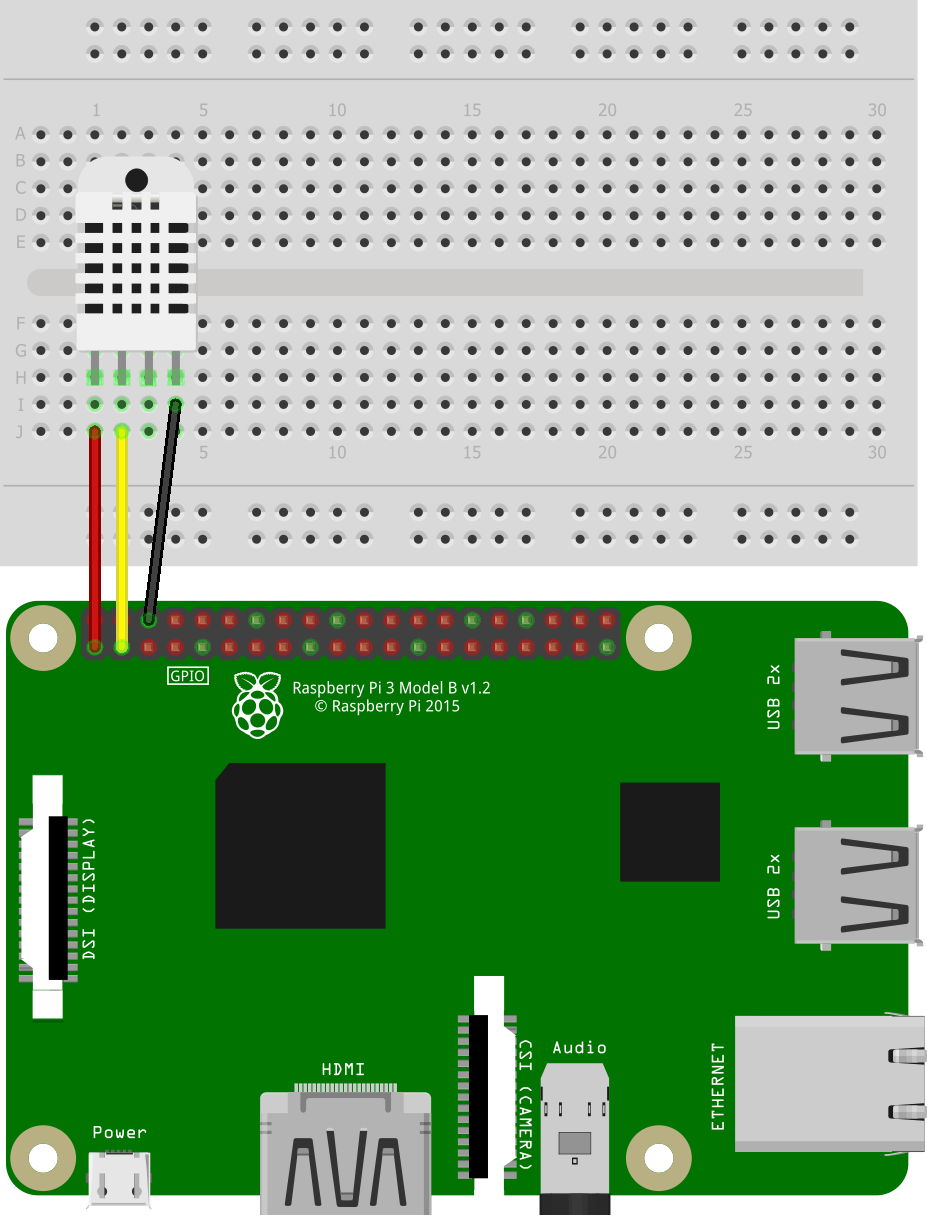
\includegraphics[scale=0.7]{gfx/RaspberrySensorNode} 
\bigskip

To interface with the sensor from the Node application, a npm package called node-dht-sensor needed to be added to the project.

The Nodejs application for the BLE node is structured as shown in the following diagram. For each of the components, the most important public methods are shown in order to show the interfacing between them. Private methods and members are not included to maintain the simplicity of the diagram.

\bigskip
\includegraphics[scale=0.6]{gfx/bleNode_Architecture} 
\bigskip

For each file, a short description of its purpose is provided.
\begin{itemize}
\item bleAdvertiser - class used for handling the BLE broadcasting. The sensor id and status code are broadcasted as the name of the device, separated by a semi-column. As the maximum name size allowed is 31 bytes, this field is more than enough for the information we require to make public. The class has only one public method that takes as argument the status code to broadcast.
\item restClient - class incorporating the logic and callbacks for making rest API calls over the network. This class exposes one public method used by the application to report the status and sensor data to the main server.
\item sensorInterface - class constantly pooling the data from the sensor and providing it when needed to the main application logic. This class is using an internal timer to control the frequency of poling sensor data.
\item utils - class containing helper methods used by the other components in the application. In this class, one method for comparing two different instances of sensor data in json format is provided. This is required to prevent the node from sending redundant data to the main server.
\item app - this is the main class of the application. It incorporates the rules and conditions for determining the status codes and uses most of the other classes, each having a specific role.
\item globals - class used for holding a set of global variables used throughout the application. The containing json file can therefore be used as application configuration that has different contents depending on the deployment sensor nodes.
\end{itemize}

The BLE node is designed to call only one REST method on the main server - reportStatus. This has been however thought so the sensor can both report data and aliveness. The sensor therefore calls the method each time the data or sensor status changes. If the measured values are constant, a call will be made every minute. This ensures that the time interval between 2 sensor updates is 60 seconds or less. Using this approach allows the server to determine whether the sensor is no longer active/connected to the network and inform the users accordingly. 




\section {Android node}
\label {Impl_AndroidNodeSection}

Write here...



%%% Local Variables:
%%% mode: latex
%%% TeX-master: "../ClassicThesis"
%%% End:
